\documentclass[border=4pt]{standalone}
\usepackage[T1]{fontenc}
\usepackage{lmodern}
\usepackage{amsmath}
\usepackage{pgfplots}
\pgfplotsset{compat=1.18}
\usepgfplotslibrary{groupplots,fillbetween}
\usetikzlibrary{calc,arrows.meta}
% one colour per kind of method, the same in every figure (Okabe-Ito)
\definecolor{neur}{HTML}{D55E00}   % neurons chosen by attribution
\definecolor{dirc}{HTML}{009E73}   % directions from the weird-vs-normal contrast
\definecolor{read}{HTML}{0072B2}   % readout methods and interventions chosen from readouts
\definecolor{pers}{HTML}{CC79A7}   % Assistant Axis / persona
\definecolor{ctrl}{HTML}{8C8C8C}   % random controls
\definecolor{meas}{HTML}{E69F00}   % measured outcome
\definecolor{ink}{HTML}{222222}
\pgfplotsset{
  every axis/.append style={clip=false, font=\small, axis line style={black!55}, tick style={black!55}, tick align=outside,
    label style={font=\small}, tick label style={font=\footnotesize}, title style={font=\small, align=center}},
  grid style={black!9, line width=0.4pt},
  every axis legend/.append style={font=\footnotesize, draw=none, fill=none},
  ci/.style={/pgfplots/error bars/x dir=both, /pgfplots/error bars/x explicit, /pgfplots/error bars/error bar style={line width=0.8pt}, /pgfplots/error bars/error mark=none},
  yci/.style={/pgfplots/error bars/y dir=both, /pgfplots/error bars/y explicit, /pgfplots/error bars/error bar style={line width=0.8pt}, /pgfplots/error bars/error mark=none},
}

\begin{document}
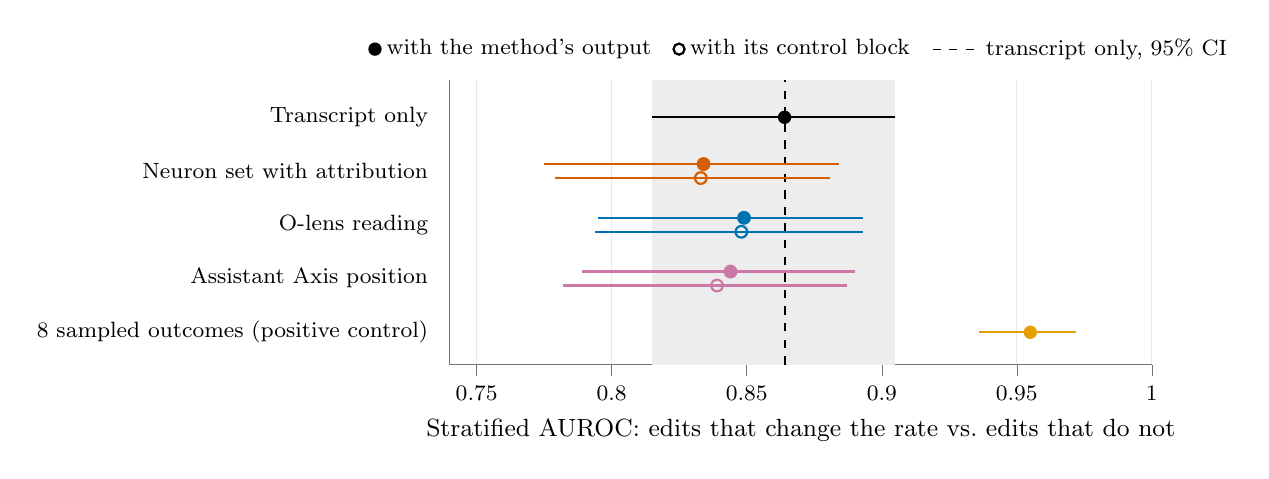
\begin{tikzpicture}
\begin{axis}[width=10.5cm, height=5.2cm, xmin=0.74, xmax=1.0, xtick={0.75,0.8,0.85,0.9,0.95,1.0}, xticklabel style={/pgf/number format/.cd, fixed, precision=2}, ymin=-4.6, ymax=0.7,  yticklabels={Transcript only,Neuron set with attribution,O-lens reading,Assistant Axis position,8 sampled outcomes (positive control)}, ytick={0,-1,-2,-3,-4}, y tick label style={font=\footnotesize}, major y tick style={draw=none}, axis x line*=bottom, axis y line*=left, xmajorgrids, xlabel={Stratified AUROC: edits that change the rate vs.\ edits that do not}, legend style={at={(0.5,1.03)}, anchor=south, legend columns=3, /tikz/every even column/.append style={column sep=6pt}}, legend cell align=left]
\fill[black!7] (axis cs:0.815,-4.6) rectangle (axis cs:0.905,0.7);
\draw[black, dashed, line width=0.7pt] (axis cs:0.864,-4.6) -- (axis cs:0.864,0.7);
\addlegendimage{only marks, mark=*, mark size=2.2pt, black}\addlegendentry{with the method's output}
\addlegendimage{only marks, mark=o, mark size=2pt, black, line width=0.8pt}\addlegendentry{with its control block}
\addlegendimage{dashed, black}\addlegendentry{transcript only, 95\% CI}
\addplot[only marks, mark=*, mark size=2.2pt, black, ci, forget plot] coordinates {(0.864,0) += (0.041,0) -= (0.049,0)};
\addplot[only marks, mark=*, mark size=2.1pt, neur, line width=0.8pt, ci, forget plot] coordinates {(0.834,-0.87) += (0.050,0) -= (0.059,0)};
\addplot[only marks, mark=o, mark size=2.1pt, neur, line width=0.8pt, ci, forget plot] coordinates {(0.833,-1.13) += (0.048,0) -= (0.054,0)};
\addplot[only marks, mark=*, mark size=2.1pt, read, line width=0.8pt, ci, forget plot] coordinates {(0.849,-1.87) += (0.044,0) -= (0.054,0)};
\addplot[only marks, mark=o, mark size=2.1pt, read, line width=0.8pt, ci, forget plot] coordinates {(0.848,-2.13) += (0.045,0) -= (0.054,0)};
\addplot[only marks, mark=*, mark size=2.1pt, pers, line width=0.8pt, ci, forget plot] coordinates {(0.844,-2.87) += (0.046,0) -= (0.055,0)};
\addplot[only marks, mark=o, mark size=2.1pt, pers, line width=0.8pt, ci, forget plot] coordinates {(0.839,-3.13) += (0.048,0) -= (0.057,0)};
\addplot[only marks, mark=*, mark size=2.2pt, meas, ci, forget plot] coordinates {(0.955,-4) += (0.017,0) -= (0.019,0)};
\end{axis}
\end{tikzpicture}
\end{document}
